%%%%%%%%%%
%
% Section: 3.2 Quadratic Equations, Functions, Zeros, and Models
% Author: John Hammond
%
%%%%%%%%%%

%%
%% Directions:
%% 1. Update the section's title and your name above
%% 2. Begin your edits beneath the %%%%%%%%% BEGIN HERE %%%%%%%%% line
%%
%% You can define terms like:
%% A \underline{quadratic equation} is an equation of the form \lgblank, where $a\ne 0$, and $a, b, c \in \mathbb{R}$. 
%%
%% Examples are of the form:
%% \begin{examples}[Directions here. Can be blank.]
%%   \ex This is an example \\[1in]     % it is up to you to specify appropriate spacing 
%% \end{examples}
%%
%%
\documentclass[11pt]{article}
\usepackage{workbook}
\begin{document}
%\tocsection{3.2:  Quadratic Equations, Functions, Zeros, and Models}
\thispagestyle{empty}
\sffamily

\noindent
\begin{center}
\huge 3.2:  Quadratic Equations, Functions, Zeros, and Models\normalsize

\rule{7in}{2pt}
\end{center}

%%%%%%%%%%% BEGIN HERE %%%%%%%%%%%%%%%%%

\noindent \underline{\textbf{Quadratic Equations and Functions:}} \\[0.15in]
A \underline{quadratic equation} is an equation of the form \lgblank, where $a\ne 0$, and $a, b, c \in \mathbb{R}$. \\[.15in]
A \underline{quadratic function} is a function of the form \lgblank, where $a\ne 0$, and $a, b, c \in \mathbb{R}$. \\[.15in]
Solving a quadratic equation is equivalent to finding the zeros of a quadratic function. \\[.15in]
\framebox{
\begin{tabular}{p{1in}|c|c|c}
\textbf{Graphs:}  &
 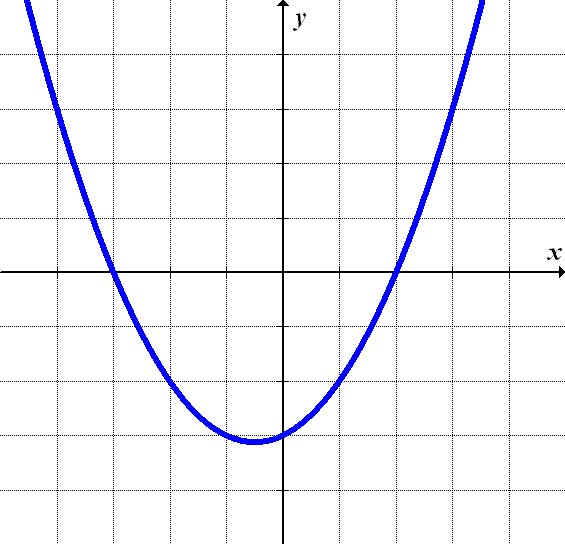
\includegraphics[width=1.75in]{parabola2.png} &
 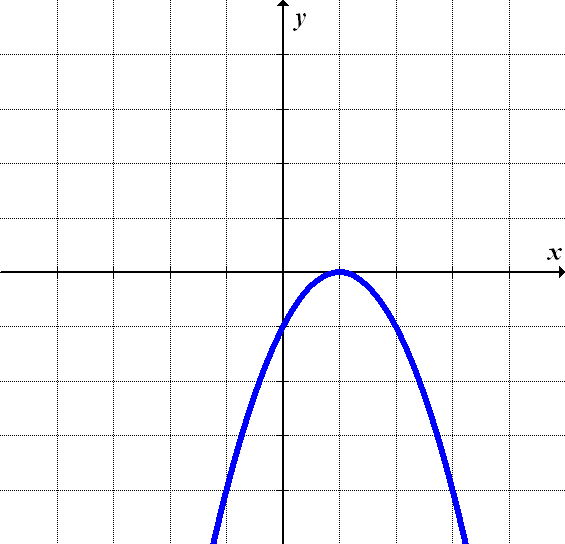
\includegraphics[width=1.75in]{parabola1.png} &
 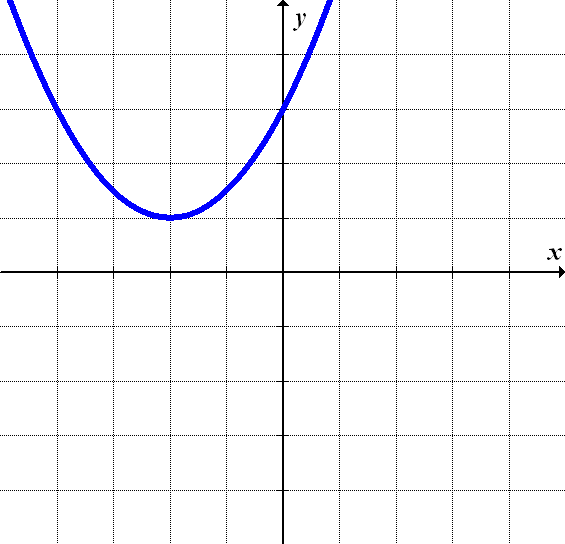
\includegraphics[width=1.75in]{parabola0.png} \\ \hline 
& & & \\[-.1in]
\textbf{\# of $x$-int:} & & & \\ \hline
& & & \\[-.1in]
\textbf{\# of zeros:} & & & \\ \hline
& & & \\[-.1in]
\textbf{Discriminant:} & & & \\ \hline
 & & & \\[-.1in]
\textbf{Solutions:} & & & \\
\end{tabular}}

\begin{verbatim}
\begin{examplestwocolumns}{This is having two columns}
  \ex $x^2-2x+4=0$ &
  \ex $5t^2-7t=0$ \\[.5in]
\end{examplestwocolumns}
\end{verbatim}
\begin{examplestwocolumns}{This is having two columns}
  \ex $x^2-2x+4=0$ &
  \ex $5t^2-7t=0$ \\[.5in]
\end{examplestwocolumns}

\noindent \underline{\textbf{Solving Quadratic Equations:}} 
We will employ three methods for solving quadratic equations:
\begin{enumerate}
\item FACTORING
\begin{examples}{Solve by factoring:}
  \ex $5t^2-7t=0$ \\[.75in]
  \ex  $3x^2+x-2=0$ \\[.75in]
  \ex $x^2+4x=-4$ \\[.75in]
\end{examples}
\begin{verbatim}
\begin{examples}{Solve by factoring:}
  \ex $5t^2-7t=0$ \\[.75in]
  \ex  $3x^2+x-2=0$ \\[.75in]
  \ex $x^2+4x=-4$ \\[.75in]
\end{examples}
\end{verbatim}
% \item COMPLETING THE SQUARE

% Recall that $(x+A)^2 = x^2 + 2Ax + A^2$ is a perfect square trinomial.  Suppose we have an expression such as $x^2+18x$, and we want to add a constant so that it creates a perfect square:

% $$x^2+18x+\xsblank = (\smblank)^2$$

% \begin{examples}[Solve by completing the square:]
%   \ex $x^2-4x+2=0$ \\[1in]
%   \ex $t^2+3t-7=0$ \\[1in]
%   \ex $3x^2-6x-4=0$\\[1in]
%   \ex $2z^2+3z-2=0$\\[1in]
% \end{examples}
% \item THE QUADRATIC FORMULA (developed by completing the square on $ax^2+bx+c=0$)\\[.25in]
% $$x=\lgblank$$

 \end{enumerate}

\subsection*{Equations Reducible to Quadratic}


\begin{verbatim}
\begin{examplesthreecolumns}{This is a three column example}
  \ex $x^2-2x+4=0$ &
  \ex $2x^2 - 3=0$ &
  \ex $5t^2-7t=0$ \\[.5in]
\end{examplesthreecolumns}
\end{verbatim}
\begin{examplesthreecolumns}{This is a three column example}
  \ex $x^2-2x+4=0$ &
  \ex $2x^2 - 3=0$ &
  \ex $5t^2-7t=0$ \\[.5in]
\end{examplesthreecolumns}

\end{document}

